\documentclass[main]{subfiles}
\begin{document}

%@@@@@@@@@@@@@@@@@@@@@@@@@@@@@@
% summarizes lecture 
% author:

\section{Design of Linear Discriminant Functions}
Linear discriminant analysis (LDA) as in  the related Fisher's linear discriminant are methods used in statistics, pattern recognition and machine learning to find a linear combination of features which characterizes or separates two or more classes of objects or events. The resulting combination may be used as a linear classifier, or, more commonly, for dimensionality reduction before later classification. (Wikipedia, Linear Discriminant Analysis \url{https://en.wikipedia.org/wiki/Linear_discriminant_analysis}.

\subsection{Generalized Linear Discriminant Functions}
\[\pl{g(x) = w_0 + \sum\limits_{i \leq d} w_ix_i  = \overbrace{(w_0,w)}^{\hidewidth\text{generalized coords a}\hidewidth}\underbrace{(1,x)^T}_{\hidewidth\text{generalized coords }\tilde x\hidewidth} = a^T\tilde x}\]
Quadratic Discriminant Functions:
\[\pl{g(x) = w_0 + \sum\limits_{i \leq d} w_ix_i + \sum\limits_{i \leq d}\sum\limits_{j \leq d} w_{ij}x_ix_j}\]
\subsubsection{How to learn nonlinear discriminant functions?}
Transform the features non-linearly and use the linear classifier in a high dimensional feature space as usual.
\begin{figure}[H]
\centering
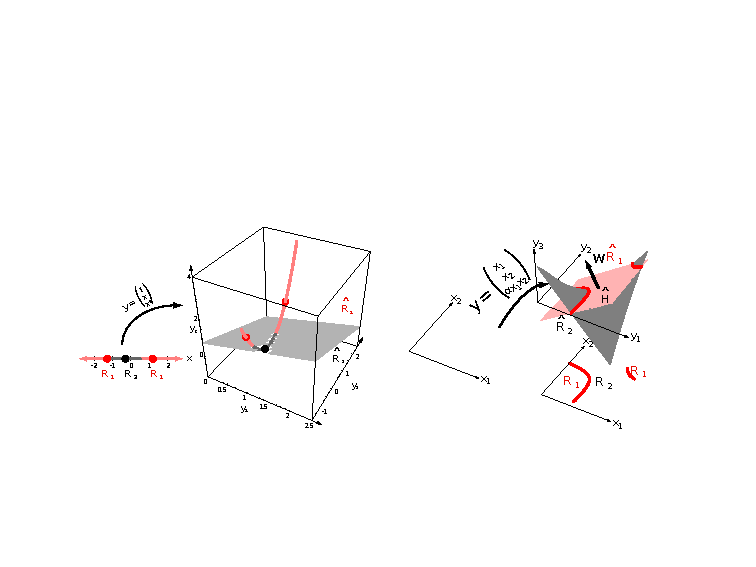
\includegraphics[trim=2cm 2cm 1.5cm 2cm, clip=true, width=0.8\linewidth]{figs/non-linear-classification-.pdf}
\end{figure}
\subsubsection{Advantage of Homogeneous Coordinates}
\[\pl{\tilde{x} = (1,x)^T ~~ a = (w_0,w)^T}\]
Easy transform, but makes analysis much easier.
\begin{enumerate}
\item Class 1 if \(\pl{a^T\tilde{x_i} > 0}\)
\item Class 2 if \(\pl{a^T\tilde{x_i} < 0}\)
\end{enumerate}
\paragraph{Normalization} transform \(\pl{\tilde{x_i} \rightarrow - \tilde{x_i}}\) iff the object belongs to class 2.

\todo[inline]{Why would you do that?Maybe to let data from class 2 get properties of class 1...}

\subsubsection{Linearly separable two class case}
Linear separability
\[\pl{\exists a \text{ with } 
\begin{cases}
a^T\tilde{x_i} > 0 & \mbox{for } y_i = 1\\
a^T\tilde{x_i} < 0 & \mbox{for } y_i = 2\\
\end{cases}}\]
\begin{itemize}
\item Problem: The solution vector is not unique.
\item Idea: Introduce a margin \(b\) to classify data with a "safe" distance from the decision boundary, i.e. \(\pl{a^T\tilde{x_i} \geq b > 0} ~ \rightarrow\) regularization of the classifier!
\end{itemize}

\todo[inline]{Why is the solution vector not unique? Because it is more of a region?Then the idea does not make sense.}

\subsubsection{Gradient descent}
\(J(a(k))\) is a general cost function for weight vector \(a\). It measures how
well a hyperplane orthogonal to \(a\) classifies the data.
\(\pl{\eta(k)}\) denotes the step size or learning rate at iteration \(k\).

\begin{enumerate}[itemsep=-0.5ex]
\item init \(a,\epsilon,\eta(\cdot),k=0\)
\item \textbf{repeat}
\item \hspace{0.5em} \(\pl{a = a + \eta(k)\nabla J(a)}\)
\item \hspace{0.5em} \(\pl{k = k + 1}\)
\item \textbf{until} \(\pl{|\eta(k)\nabla J(a)| < \epsilon}\)
\end{enumerate}
Best learning rate is \(\eta^{opt} = \frac{||\nabla J||^2}{\nabla J^T\frac{\partial^2J}{\partial a_i\partial a_j}\nabla J}\)\\
(2nd order taylor expansion of \(J(a)\) at \(a(k)\) then insert gradient descent rule \(\pl{a(k + 1) - a(k) = -\eta(k)\nabla J(a(k))}\))
\subsubsection{Newton's Algorithm}
Optimality Condition: Choose \(a(k + 1)\) to minimize the \(2^{nd}\) order Taylor expansion of \(J(a(k + 1))\), i.e.
\begin{align}
\pl{
\frac{\partial}{\partial a(k+1)}J(a(k+1)) &= 0\\
\nabla J + \frac{\partial^2J}{\partial a_i\partial a_j}(\underbrace{a(k+1)-a(k)}_{-\eta\nabla J}) &= 0\\
\eta\nabla J &= H^{-1}\nabla J\\
}
\end{align}
Newton's Descent Rule: \(\pl{a(k+1) = a(k)-H^{-1}\nabla J}\)
\begin{enumerate}[itemsep=-0.5ex]
\item init \(a,\epsilon,\eta(\cdot),k=0\)
\item \textbf{repeat}
\item \hspace{0.5em} \(\pl{a = a - \underline{H^{-1}\nabla J}}\)
\item \hspace{0.5em} \(\pl{k = k + 1}\)
\item \textbf{until} \(\pl{|\eta(k)\nabla J(a)| < \epsilon}\)
\end{enumerate}
\begin{figure}[H]
\centering
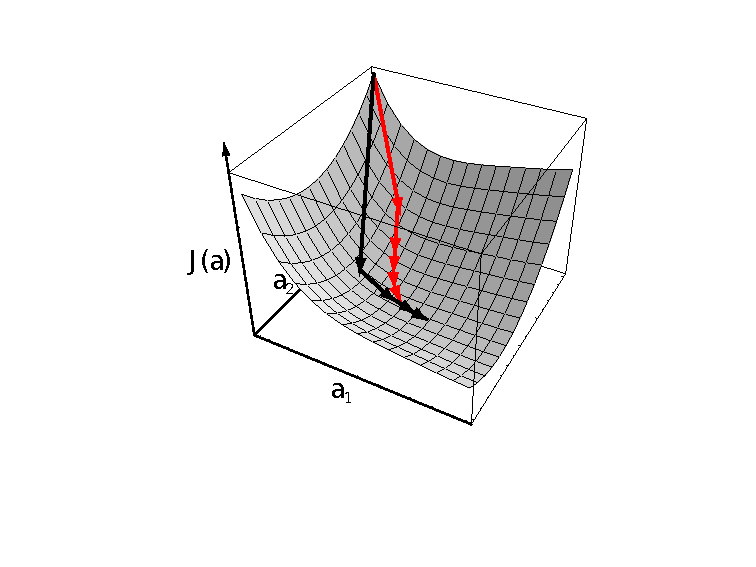
\includegraphics[trim=1.5cm 1.5cm 1.5cm 1cm, clip=true,width=0.6\linewidth]{figs/newton-naive-gd}
\caption{The sequence of weight vectors given by a simple gradient descent (red) and by Newton’s (second order) gradient algorithm (black). Newton’s rule leads to greater improvement per step, even when using optimal learning methods. However added computational burden of inverting the Hessian matrix.}
\end{figure}

\subsection{Perceptrons}
We need a cost function \(\pl{J(a,\tilde{x_1},\ldots,\tilde{x_n}}\), that qualifies as a good cost function to update the weights and to solve the inequalities \(\pl{a^T\tilde{x_i} > 0,~\forall i}\).
\begin{enumerate}
\item Number of misclassified samples is not a good choice as it is piecewise constant and without gradient.
\item Sum of violating projections
\[\pl{
J_p(a) = \sum\limits_{\tilde{x} \in \underbrace{\tilde{\mathcal{X}}}_{\hidewidth\text{set of missclassified samples}\hidewidth}}(-a^T\tilde{x})}\]
Perceptron Rule: \(\pl{a(k+1) = a(k) + \eta(k)\sum\limits_{\tilde{x}\in\tilde{\mathcal{X}}} \tilde{x}}\)
\end{enumerate}
Batch version with variable learning rate:
\begin{enumerate}[itemsep=-0.5ex]
\item init \(a,\epsilon,\eta(\cdot),k=0\)
\item \textbf{repeat}
\item \hspace{0.5em} \(\pl{a = a + \underline{\sum\limits_{\tilde{x}\in \tilde{\mathcal{X}}}\eta (k)\tilde{x}}}\)
\item \hspace{0.5em} \(\pl{k = k + 1}\)
\item \textbf{until} \(\pl{|\eta(k)\sum\limits_{\tilde{x}\in \tilde{\mathcal{X}}}| < \epsilon}\)
\end{enumerate}
Fixed-Increment Single Sample Perceptron (moves the solution vector hyperplane towards the misclassified samples to make them switch sides):
\begin{enumerate}[itemsep=-0.5ex]
\item init \(a,\eta(\cdot),k=0\)
\item \textbf{repeat}
\item \hspace{0.5em} \(\pl{k = k + 1 \mod n}\)
\item \hspace{0.5em} \textbf{if} \(\pl{\tilde{x}^k}\) is misclassified by \(a\) \textbf{then}
\item \hspace{1em} \(\pl{a = a + \underline{\tilde{x}^k}}\)
\item \hspace{0.5em} \textbf{end if}
\item \textbf{until} all patterns are correctly classified
\end{enumerate}
\subsubsection{Convergence of the perceptron rule}
If the training samples are linearly separable, then the
sequence of weight vectors \(\pl{a = a + \tilde{x^k}}\) will terminate at a
solution vector.
\todo[inline]{Make proof easy to understand.}
\subsubsection{Limitations of Single-Layer Perceptron}
A single-layer perceptron can not solve the XOR problem.
\begin{figure}[H]
\centering
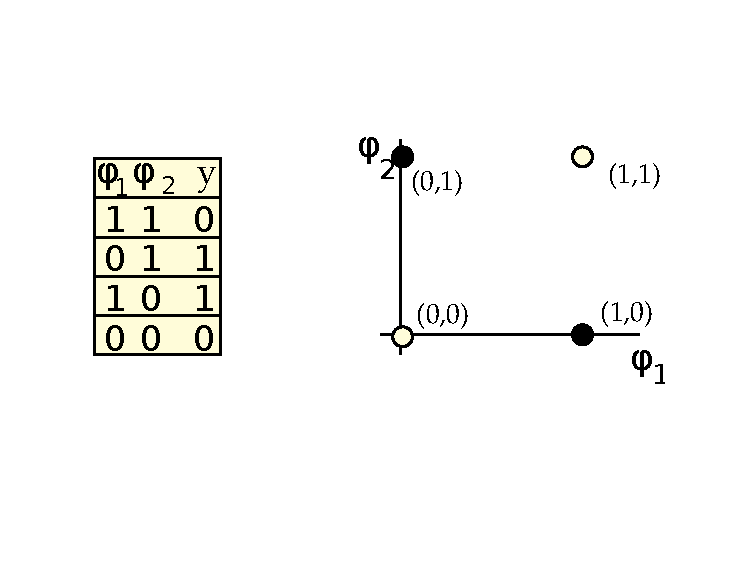
\includegraphics[width=0.6\linewidth]{figs/XOR-problem.pdf}
\caption{The XOR data set as shown here can not be separated in a 2 dimensional setting. Therefore, the single-layer perceptron can not achieve a proper separation. With a multilayer perceptron, we can get this data set into higher dimensions to make it properly separable.}
\end{figure}
Variable-Increment Perceptron with Margin
\begin{enumerate}[itemsep=-0.5ex]
\item init \(a,\epsilon,\eta(\cdot),k=0\)
\item \textbf{repeat}
\item \hspace{0.5em} \(\pl{k = k + 1}\)
\item \hspace{0.5em} \textbf{if} \(\pl{a^T\tilde{x^k} \leq b}\) \textbf{then}
\item \hspace{1em} \(\pl{a = a + \underline{\eta(k) \tilde{x}^k}}\)
\item \hspace{0.5em} \textbf{end if}
\item \textbf{until} \(\pl{a^T\tilde{x^k}>b, \forall k}\)
\end{enumerate}
\todo[inline]{We do not need the threshold\(\epsilon\) here!}
We can formulate all perceptron algorithms as batch (all-data-at-once) or online (sequential data processing) algorithms. Online variance have a dependency on the sequence but tend to be more robust.
\todo[inline]{Why are they more robust?}
\subsection{WINNOW algorithm}
Idea: Exponential update of weights\\
Consider a two class learning problem with many irrelevant
dimensions (normalization is not performed).
\begin{enumerate}
\item \(a^+ , a^-\) are weight vectors associated with either class and are corrected iff samples of their class are misclassfied.
\item \(\alpha\) is the scaling factor for exponential update.
\item \(z_k =
\begin{cases}
1 & \mbox{if } \tilde{x_k} \text{ belongs to class 1}\\
-1 & \mbox{if } \tilde{x_k} \text{ belongs to class 2}\\
\end{cases}
\)
\end{enumerate}

Balanced WINNOW
\begin{enumerate}[itemsep=-0.5ex]
\item init \(a^+,a^-,\epsilon,\eta(\cdot),k=0,\alpha > 1\)
\item \textbf{repeat}
\item \hspace{0.5em} \(\pl{k = k + 1 \mod n}\)
\item \hspace{0.5em} \textbf{if} \(\pl{\sgn[a^{+T},a^{-T}\tilde{x_k}] \neq z_k}\) \textbf{then} (pattern misclassified)
\item \hspace{1em} \textbf{if} \(\pl{z_k = +1}\) \textbf{then} (class 1 error)
\item \hspace{1.5em} \textbf{for all } \(i \leq d\) \textbf{do}
\item \hspace{2em} \(\pl{a^+_i = a^+_i \cdot \alpha^{+\tilde{x_{ki}}}} \) (exponentiated update)
\item \hspace{2em} \(\pl{a^-_i = a^-_i \cdot \alpha^{-\tilde{x_{ki}}}} \)
\item \hspace{1.5em} \textbf{end for}
\item \hspace{1em} \textbf{end if}
\item \hspace{1em} \textbf{if} \(\pl{z_k = -1}\) \textbf{then} (class 2 error)
\item \hspace{1.5em} \textbf{for all } \(i \leq d\) \textbf{do}
\item \hspace{2em} \(\pl{a^+_i = a^+_i \cdot \alpha^{-\tilde{x_{ki}}}} \) (exponentiated update)
\item \hspace{2em} \(\pl{a^-_i = a^-_i \cdot \alpha^{+\tilde{x_{ki}}}} \)
\item \hspace{1.5em} \textbf{end for}
\item \hspace{1em} \textbf{end if}
\item \hspace{0.5em} \textbf{end if}
\item \textbf{until} convergence
\end{enumerate}
\subsubsection{Minimum squared error procedures}
\paragraph{Closed form solution}
LSE learning is learning with all \(\pl{\tilde{x_i}}\) in \(\pl{a^T\tilde{x_i}  = b_i > 0}\) instead of training it with \(\pl{\tilde{x_i} \in \tilde{\mathcal{X}}}\) in \(\pl{a^T\tilde{x_i} > 0~\forall i}\)
As we have the learning condition as \(\pl{\tilde{X}a = b}\), we can get the error criterion as \(e = \tilde{X}a - b\). The squared error is then 
\[\pl{J_s(a) = ||\tilde{X}a-b||^2 = \sum\limits_{i\leq n}(a^T\tilde{x_i}-b_i)^2}\]
from this we can calculate the gradient by deriving it:
\[\pl{\nabla J_s = 2 \tilde{X}^T(\tilde{X}a-b) = 0 \rightarrow a = (\tilde{X}^T\tilde{X})^{-1}\tilde{X}^Tb = \underbrace{\tilde{X}^\dagger}_{\hidewidth\text{pseudo inverse of }\tilde{X}\hidewidth} b}\]
\paragraph{Iterative solution}

\begin{enumerate}[itemsep=-0.5ex]
\item init a(1)
\item \textbf{repeat}
\item \hspace{0.5em}\(\pl{\eta(k) = \frac{\eta(1)}{k}}\)
\item \hspace{0.5em} \(\pl{a(k+1) = a(k) - \frac{\eta(k)}{2} \nabla J_s}\)\(~~~~(\pl{= a(k) - \eta(k)\tilde{X}^T(\tilde{X}a(k)-b)})\)
\item \textbf{until} convergence
\end{enumerate}
\subsubsection{LMS Rule}
\begin{enumerate}[itemsep=-0.5ex]
\item init \(\pl{a, b, \theta, \eta(\cdot)}\)
\item k = 0
\item \textbf{repeat}
\item \hspace{0.5em} \(\pl{k = k + 1 \mod n}\)
\item \hspace{0.5em}\(\pl{\eta(k) = \frac{\eta(1)}{k}}\)
\item \hspace{0.5em} \(\pl{a = a + \underline{\eta(k) (b_k a^T\tilde{x}^k)\tilde{x}}^k}\)
\item \textbf{until} \(\pl{|\eta(k)(b_k - a^T \tilde{x}^k ) \tilde{x}^k | < \theta }\)
\end{enumerate}
\subsection{Fisher's linear discriminant analysis}
\textbf{Idea:} Project high-dimensional data of two classes to a one-dimensional linear subspace such that the classes are optimally separated.

\begin{figure}[H]
\centering
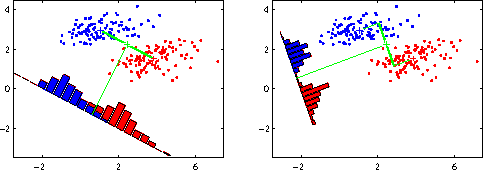
\includegraphics[width=0.8\linewidth]{figs/fishers-linear-discriminant-analysis.pdf}
\caption{Projection on the left is suboptimal as it does not separate the classes properly, whereas the projection on the right gives rise to proper class separations.}
\end{figure}

We have samples \(\pl{\mathcal{Z} = \{(x_1,y_1),\ldots,(x_n,y_n)\} =: \mathcal{X} \times \mathcal{Y}}\) that we want to partition into k class specific subsets \(\pl{\mathcal{Z}_{y_i} = \mathcal{X}_{y_i} \times \mathcal{Y}_{y_i},~1 \leq y_i \leq k,~\forall x_i \in \mathcal{X}_{y_i} }\) by a projection \(\pl{x'_i = w^Tx_i,~1 \leq i \leq n}\).\\
\subsubsection{How to we measure the discrimination of the projected points?}
\paragraph{Sample averages (class centroids):} 
\[\pl{m_{y_i} = \frac{1}{\underbrace{n_{y_i}}_{|\mathcal{X}_{y_i}|}} \sum\limits_{x\in\mathcal{X}_{y_i}}x}\]

\paragraph{Averages of projected points:}
\[\pl{m_{y_i} = \frac{1}{\underbrace{n_{y_i}}_{|\mathcal{X}_{y_i}|}} \sum\limits_{x\in\mathcal{X}_{y_i}}w^Tx=w^Tm_{y_i}}\]
 
\paragraph{Distance of the sample averages in the two class case:}
\[w^T(m_1-m_2)\]

\paragraph{Scatter of class \(y_i\):}
\[\pl{\Sigma_{y_i} = \sum\limits_{x\in\mathcal{X}_{y_i}}(x-m_{y_i})(x-m_{y_i})^T}\]

\paragraph{"Within" scatter:}
\[\pl{\Sigma_{w} = \Sigma_1 + \Sigma_2}\]

\paragraph{Scatter of projected data(average of class specific variance)}
\begin{align}
\pl{
\tilde{\Sigma}_{y_i} &= \sum\limits_{x\in\mathcal{X}_{y_i}}(w^Tx-\tilde{m}_{y_i})(w^Tx-\tilde{m}_{y_i})^T\\
&= \sum\limits_{x\in\mathcal{X}_{y_i}}w^T(x-m_{y_i})(x-m_{y_i})^Tw\\
&=w^T\Sigma_{y_i}w\\
\text{Two classes: }\rightarrow \tilde{\Sigma}_1 + \tilde{\Sigma}_1 &= w^T\Sigma_ww
}
\end{align}
\textbf{Remark:} To separate the data of different classes as good as possible, the class centroids in the projected space should be as far away as possible and, simultaneously, the variance in the projection space of the class specific data should be as small as possible.
\subsubsection{Separation Criterion}
\textbf{Idea:} Separate classes as good as possible relative to their variances (maximal J(w) = optimal w)
\[\pl{J(w) = \frac{\sigma^2_{between}}{\sigma^2_{within}} = \frac{||\tilde{m}_1-\tilde{m}_2||^2}{\tilde{\Sigma}_1 + \tilde{\Sigma}_2} = \frac{w^T\overbrace{(m_1-m_2)(m_1-m_2)^T}{=\Sigma_B}w}{w^T\Sigma_Ww}}\]
So we differentiate \(J(w)\):
\begin{align}
\pl{
\frac{d}{dw} J(w) &= \frac{d}{dw} ((w^T\Sigma_Ww)^{-1}w^T\Sigma_Bw)\\
&= -2\Sigma_Ww (w^T\Sigma_Ww)^{-2}w^T\Sigma_Bw + 2(w^T\Sigma_Ww)^{-1}\Sigma_Bw = 0\\
\rightarrow \Sigma_Bw &= \Sigma_w w \frac{w^T\Sigma_Bw}{w^T\Sigma_Ww}
}
\end{align}
\paragraph{Solution via eigenvalue problem for weight vector}
\[\pl{\Sigma^{-1}_W \underbrace{\Sigma_Bw}_{\hidewidth\text{ an unscaled projector making any vector parallel to} (m_1-m_2)\hidewidth} = \lambda w,~\lambda = \frac{w^T\Sigma_Bw}{w^T\Sigma_Ww}}\]
\paragraph{Unscaled solution} \((\mathcal{O}(d^2n)\):
\[\tilde{w} = \Sigma^{-1}_W(m_1-m_2)\]
\subsubsection{Multiple Discriminant Analysis}
\begin{figure}[H]
\centering
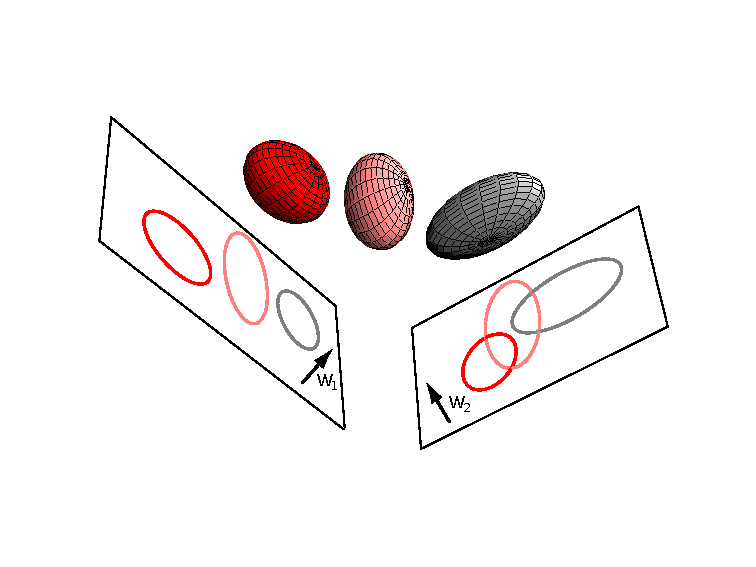
\includegraphics[width=0.8\linewidth]{figs/multiple-discriminant-analysis.pdf}
\caption{Informally, multiple discriminant methods seek the optimum such subspace, that is, the one with the greatest separation of the projected distributions for a given total within-scatter matrix.}
\end{figure}
\paragraph{k-Class Problem:} Find a \(k - 1\) dimensional linear subspace, which
separates the classes in an optimal fashion \((d \geq k)\).\\
\textbf{Within-class scatter:}
\[\pl{\Sigma_W = \sum\limits_{y_i\leq k}\Sigma_{y_i} = \underline{\sum\limits_{y_i\leq k}}\sum\limits_{x\in\mathcal{X}_{y_i}}(x-m_{y_i})(x-m_{y_i})^T}\]
with class centroids:
\[\pl{m_{y_i} = \frac{1}{\underbrace{n_{y_i}}_{|\mathcal{X}_{y_i}|}} \sum\limits_{x\in\mathcal{X}_{y_i}}x}\]
\paragraph{Total mean Vector:}
\[\pl{m = \frac{1}{n}\Sigma_xx = \frac{1}{n} \Sigma_{y_i}n_{y_i}m_{y_i}}\]
\todo[inline]{What is n here?Number of objects in class?}
\paragraph{Total Scatter Matrix:}
\begin{align}
\pl{
\Sigma_T &= \frac{1}{n}\Sigma_x(x-m)(x-m)^T\\
&=\sum\limits_{y_i}\sum\limits_{x\in\mathcal{X_{y_i}}}(x-m_{y_i}+m_{y_i}-m)(x-m_{y_i}+m_{y_i}-m)^T\\
&=\sum\limits_{y_i}\sum\limits_{x\in\mathcal{X_{y_i}}}(x-m_{y_i})(x-m_{y_i})^T + \sum\limits_{y_i}\sum\limits_{x\in\mathcal{X_{y_i}}}(m_{y_i}-m)(m_{y_i}-m)^T\\
&=\Sigma_W + \sum\limits_{y_i}n_{y_i}(m_{y_i}-m)(m_{y_i}-m)^T = \Sigma_W + \Sigma_B\\
}
\end{align}
Projection from a d-dimensional feature space to a (k - 1)-dimensional subspace is achieved by (k - 1) discriminant functions \(y_i = w^T_ix,~1\leq i \leq k-1\)
\paragraph{Fisher's Criterion}
\[J(W) = \frac{|W^T\Sigma_BW|}{|W^T\Sigma_WW|}\]
\begin{enumerate}
\item Solve the generalized eigenvalue problem \(\Sigma_B w_i = \lambda_i \Sigma_W w_i\) for the \((k - 1)\) largest eigenvalues by Gram-Schmidt orthonormalization.
\item \(\Sigma_B\) is a sum of k rank one (or less) matrices; at most 
\((k - 1)\) matrices are independent (center of mass constraint)
\(\rightarrow |\Sigma_B| \leq (k-1)\).
\item Isotropic case: space is spanned by the \((k - 1)\) vectors \(m_i - m\).
\end{enumerate}
\subsubsection{Remarks on Multicategory Linear Discriminants}
It is often preferable to reformulate the multiclass problem as
\((k - 1)\) "class \(y_i\) - not class \(y_i\)" dichotomies or \(k(k - 1)/2\) "class \(\alpha\) or \(\beta\)" dichotomies.\\
\textbf{Problem:} Some areas in feature space will be ambiguously classified.
\subsection{Readings}
\begin{enumerate}
\item Perceptrons: chp 5
\item Fisher's Linear Discriminant Analysis: 4.10
\item Both: chp 5.8.2
\end{enumerate} 
\end{document}